\documentclass[12pt,a4paper,titlepage]{scrartcl}

\usepackage{preamble}

\title{TP Segmentation d'images CT de foie en 2D}
\author{Saâd Aziz Alaoui, Yassine Jamoud, Samy Haffoudhi}
\date{\today}

\begin{document}

\maketitle

\section*{Introduction}

Lors de ce TP, nous allons travailler sur la segmentation d'images CT
de foie. Pour ce faire, nous allons commencer par une analyse des données
afin d'appréhender notamment la variabilité des données. Nous
implémenterons ensuite un modèle U-NET afin de réaliser la segmentation.
Enfin nous testerons le modèle et commenterons les résultats obtenus.

\section{Analyse des données}

\subsection{Les données}

La base de données est constituée en tout de 131 images CT.
Pour chaque image CT, nous disposons d'un nombre différent de coupes, toutes
de taille 64x64. En pratique, on travaille sur les données 3D avec des
coupes de taille 512x512, ces restrictions nous permettent d'accélérer
la vitesse d'entrainement pour le TP.

On s'intéresse à la partie centrale des coupes. En effet, hors de cette
section, on aurait trop de variabilité et notre modèle sera incapable
d'apprendre correctement.

Affichons un exemple de tranches (indice z minimal, centré et maximal) et
les masques correspondants.

\begin{figure}[H]
    \caption{3 tranches et les masques correspondants}
    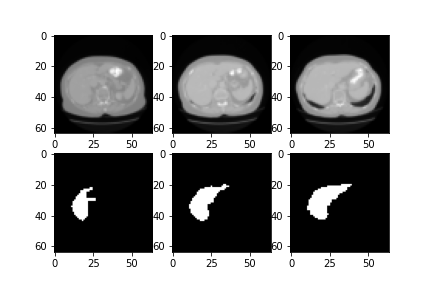
\includegraphics[width=.7\textwidth]{image_folle}
    \centering
\end{figure}

\subsection{La variabilité des données}

Afin d'appréhender la variabilité des données, affichons les intensités
moeynnes pour les 131 images CT pour les trois tranches :

\begin{figure}[H]
    \caption{Intensités moyennes}
    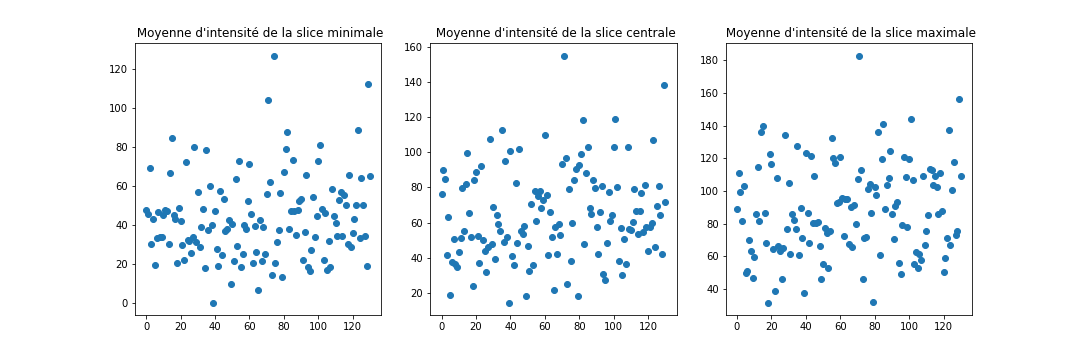
\includegraphics[width=.9\textwidth]{moyennes}
    \centering
\end{figure}

Ainsi que les volume du foie :

\begin{figure}[H]
    \caption{Volume des foies}
    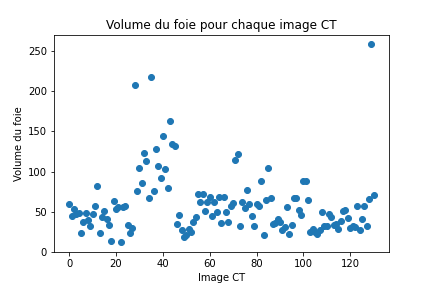
\includegraphics[width=.6\textwidth]{volumes}
    \centering
\end{figure}

Ainsi, on observe bien des variations entre les différentes images CT, ce
qui est évidemment souhaitable pour l'entrainement du modèle.

\section{Le modèle}

\subsection{Les données}

Pour construire les données \texttt{X} et les masques \texttt{Y}, on concatène les
tranches centrales de chaque image CT ainsi que les masques correspondants.

Pour réaliser le découpage entre données d'entrainement et de test,
on choisit de se baser sur le nombre d'images CT plutôt que le nombre
de tranches pour éviter le cas où on aurait trop de tranches similaires
dans un des deux ensembles ou des images trop similaires entre les
ensembles.

\subsection{Le modèle}

Nous nous intéressons ici à l'architecture \textbf{U-Net} qui permet justement d'effectuer
des taches de segmentation sémantique. Le U-net est un réseau de neurones à convolution entièrement
convolutionnel. L'idée principale derrière cette architecture est de remplacer les opérations
de pooling par des opérateurs de suréchantillonnage ce qui implique l'augmentation de de la
résolution de la sortie.

Le modèle U-net est composé d'une couche d'entrée, un encodeur et un décodeur.
L'encodeur et le décodeur ont une structure en blocs similaires mais des dimensions différentes.
Chaque bloc de l'encodeur est composé de deux couches de convolution de mêmes dimensions,
d'une couche de pooling et d'une fonction d'activation. Pour compenser la baisse de la
dimension de l'image, le nombre de filtres augmente. Enfin, le modèle dispose également d'une
liste de connexions entre l'encodeur et le décodeur.

Une visualisation de l'architecture est disponible en \textbf{annexe A}.

\subsection{L'entrainement}

On obtient les courbes d'apprentissage suivantes :

\begin{figure}[H]
    \caption{Courbes d'apprentissage}
    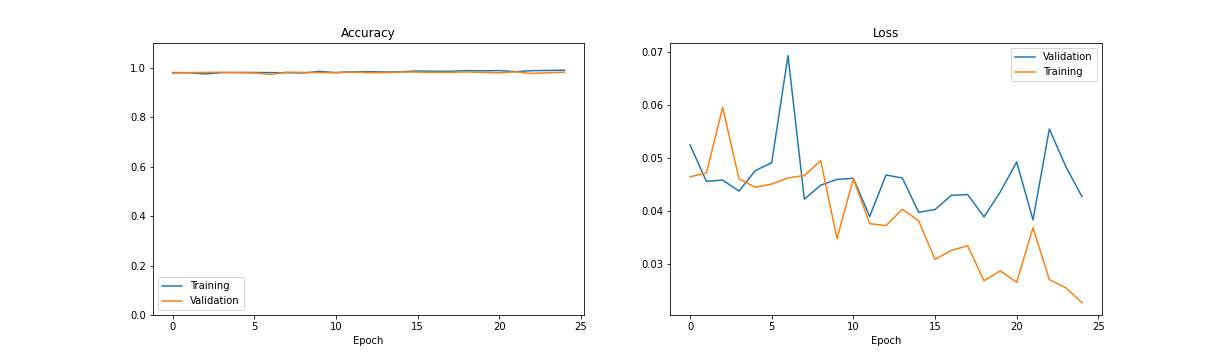
\includegraphics[width=\textwidth]{learning}
    \centering
\end{figure}

On observe que les deux courbes de précision sont très proches de 1 dès les premières itérations et restent
proches. Notre modèle apprend correctement.

\section{Résultats et tests}

On obtient un score dice moyen de 0.83, ce qui est satisfaisant. En optimisant les typer-paramètres
du modèle et en ayant par exemple recourt à de l'augmentation de données on pourrait essayer
d'augmenter ce score.

\begin{figure}[H]
    \caption{Boxplot Dice}
    \includegraphics[width=.4\textwidth]{dicescore}
    \centering
\end{figure}

Affichons les résultats obtenus pour trois tranches :

\begin{figure}[H]
    \caption{Résultats}
    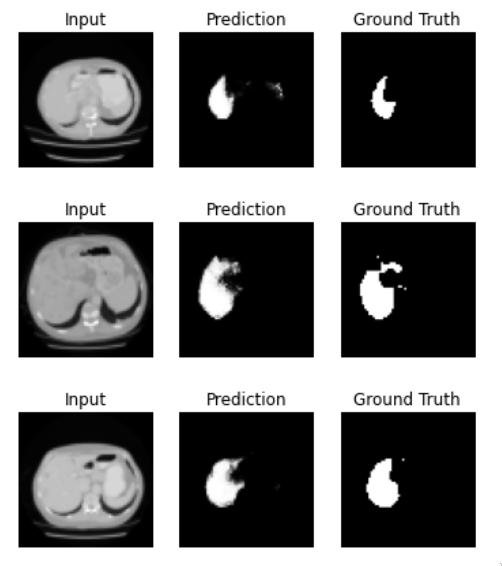
\includegraphics[width=.4\textwidth]{resultats}
    \centering
\end{figure}

On observe que les résultats sont satisfaisants pour ces différentes images. On note quand
même la présence d'artefacts par exemple visibles pour la première image et de différences aux
bords. Le travail sur notre modèle évoqué plus haut nous permettrait surement d'obtenir des résultats
encore meilleurs.

\section*{Conclusion}

Ainsi, lors de ce TP nous avons pu travailler sur le problème de la segmentation d'images CT
de foie. Bien que le cadre soit simplifié, nous avons pu découvrir le problème et ses enjeux
en comprenant les données et en mettant en place un modèle U-Net permettant de réaliser la
segmentation. Nous avons rapidement obtenu de bonne performances ce qui prouve la
puissance de telles méthodes facilitant grandement le travail des médecins.

\begin{appendices}

    \section{L'architecture du modèle}

    \begin{figure}[H]
        \caption{Architecture}
        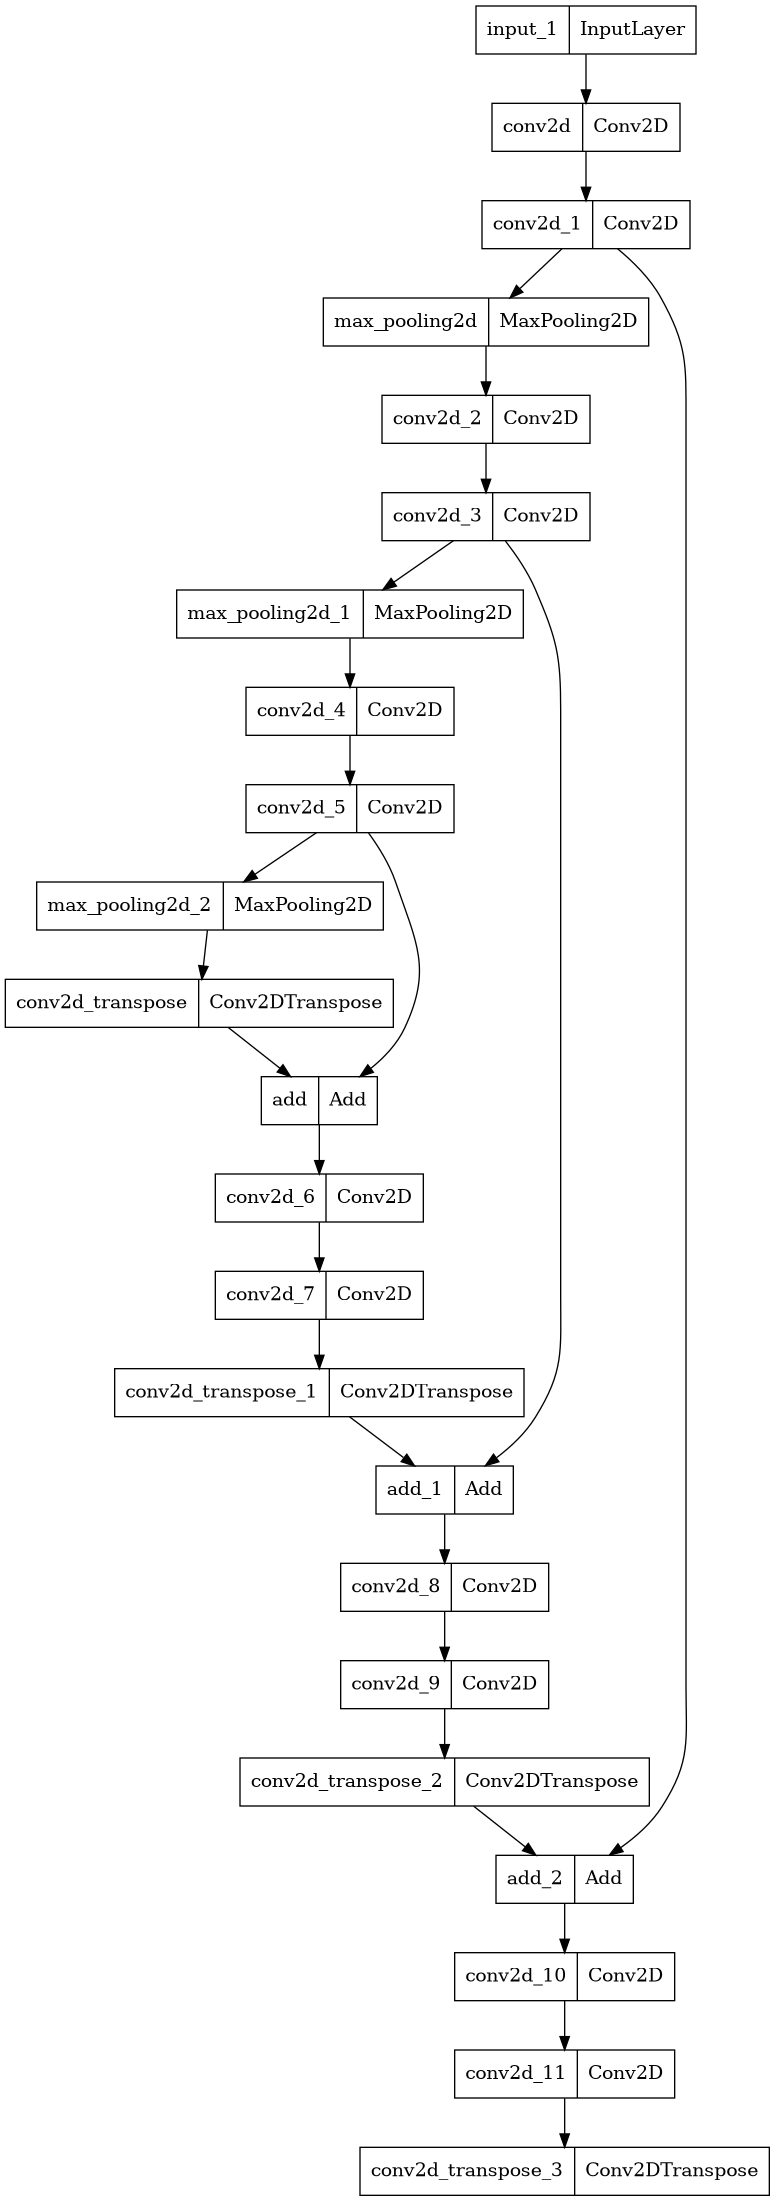
\includegraphics[width=.4\textwidth]{model}
        \centering
    \end{figure}

\end{appendices}

\end{document}
